\documentclass[10pt,xcolor=pdflatex]{beamer}
\usepackage{newcent}
\usepackage[utf8]{inputenc}
\usepackage[czech]{babel}
\usepackage{hyperref}
\usepackage{textpos}
\usepackage{multicol}
\usepackage{tikz}
\usepackage{fancyvrb}
\usepackage{color}
\usepackage{subfig}
\usepackage{geometry}
\usepackage{graphicx}
\usepackage{epstopdf}
\usepackage{todonotes}
\usepackage{listings}

\newcommand{\emp}{\lstinline[language={[LaTeX]TeX}, basicstyle=\tt\color{fitdark}]}

\lstdefinelanguage{XML}
{
  basicstyle=\ttfamily\footnotesize,
  morestring=[b]",
  moredelim=[s][\color{red}]{<}{\ },
  moredelim=[s][\color{red}]{</}{>},
  moredelim=[l][\color{red}]{/>},
  moredelim=[l][\color{red}]{>},
  morecomment=[s]{<?}{?>},
  morecomment=[s]{<!--}{-->},
  commentstyle=\color{black},
  stringstyle=\color{brown},
  identifierstyle=\color{violet}
}
\lstset{language=Java,
  showspaces=false,
  showtabs=false,
  breaklines=true,
  showstringspaces=false,
  breakatwhitespace=true,
  commentstyle=\color{green!70!black},
  keywordstyle=\color{blue},
  stringstyle=\color{red},
  basicstyle=\ttfamily,
  moredelim=[il][\textcolor{darkgrey}]{\$\$},
  moredelim=[is][\textcolor{darkgrey}]{\%\%}{\%\%}
}

\newcommand{\inlinejava}{\lstinline[language={Java}]}
\newcommand{\inlinejavaEmp}{\color{fitdark}\lstinline[language={Java}]}
\newcommand{\itmspace}[2]{\item #2 \vspace{#1}}

\epstopdfDeclareGraphicsRule{.gif}{png}{.png}{convert gif:#1 png:\OutputFile}
\AppendGraphicsExtensions{.gif}
\usetheme{FIT}

\def\uv#1{\quotedblbase#1\textquotedblleft}%
\newcommand{\putat}[3]{\begin{picture}(0,0)(0,0)\put(#1,#2){#3}\end{picture}}

%%%%%%%%%%%%%%%%%%%%%%%%%%%%%%%%%%%%%%%%%%%%%%%%%%%%%%%%%%%%%%%%%%
\title[GJA 9]{Java Persistence API and Hibernate}

\author[]{Jaroslav Dytrych}

\institute[]{Faculty of Information Technology
Brno University of Technology \\
Bo\v{z}et\v{e}chova 1/2. 612 66 Brno - Kr\'alovo Pole\\
dytrych@fit.vutbr.cz}

\date{31 October 2023}
%\date{\today}
%\date{} % bez data

%%%%%%%%%%%%%%%%%%%%%%%%%%%%%%%%%%%%%%%%%%%%%%%%%%%%%%%%%%%%%%%%%%

\begin{document}

\makeatletter
\g@addto@macro{\UrlBreaks}{\UrlOrds}
\makeatother

\frame[plain]{\titlepage}

\bluepage{Java Persistence API}

\begin{frame}\frametitle{Introduction}
	\begin{itemize}
		\item Database management
          \begin{itemize}
        	\item Java Persistence API
              \begin{itemize}
                \item uses JDBC (Java Database Connectivity)
              \end{itemize}
        	\item Object-relational mapping
        	\item Query language 
          \end{itemize}
        \medskip
		\item Entities
          \begin{itemize}
        	\item SQL tables -- Java classes
          \end{itemize}
        \medskip
		\item Fields
          \begin{itemize}
        	\item Table columns -- class properties
              \begin{itemize}
            	\item Transient -- temporary, not stored in the database
            	\item Persistent -- stored in the database
            	\item Inverse -- stored in the database in another entity table
              \end{itemize}
          \end{itemize}
	\end{itemize}
\end{frame}


\begin{frame}[fragile]\frametitle{The Minimal Entity}
    \begin{itemize}
		\item \textbf{Must be indicated as an Entity}
          \begin{itemize}
            \item \texttt{@Entity} annotation on the class
            \item[] \color{red}\verb'@Entity'\color{black}
            \item[] \verb'public class Employee { ... }'\\[.2cm]
            \item  Entity entry in XML mapping file
            \item[] \verb'<entity class="com.acme.Employee"/>'\\[0.2cm]
          \end{itemize}
        \item \textbf{Must have a persistent identifier (primary key)}
		\item[] \begin{Verbatim}[fontsize=\footnotesize, commandchars=\#\[\]]
#color[red]#textbf[@Entity]
public class Employee {
    #color[red]#textbf[@Id]#color[black] int id;
    public int getId() { return id; }
    public void setId(int id) { this.id = id; }
}
			\end{Verbatim}
	\end{itemize}
\begin{tikzpicture}[remember picture,overlay]
    \node[xshift=-0.6cm,yshift=-1.3cm] at (current page.north east){%
    
\includegraphics[width=1cm]{img/pozor}};
\end{tikzpicture}
\end{frame}


\begin{frame}[fragile]{Persistent Identity}
	\begin{itemize}
		\item Identifier (id) in entity is a primary key in the database
		\item Uniquely identifies entity in memory and in DB
		\vspace{0.25cm}
        \item Simple id -- single field/property
        \item[] \begin{Verbatim}[fontsize=\footnotesize, commandchars=$\[\]]
$color[red]$textbf[@Id]$color[black] int id;          
          	\end{Verbatim}
		\item Compound id -- multiple fields/properties
        \item[] \begin{Verbatim}[fontsize=\footnotesize, commandchars=$\[\]]
$color[red]$textbf[@Id]$color[black] int id;
$color[red]$textbf[@Id]$color[black] String name;
            \end{Verbatim}
        \item Embedded id -- single field of primary key (PK) class type
        \item[] \begin{Verbatim}[fontsize=\footnotesize, commandchars=$\[\]]
$color[red]$textbf[@EmbeddedId]$color[black] EmployeePK id;            
\end{Verbatim}
        \vspace{0.25cm}
        \item Identifiers can be generated in the database by specifying \texttt{@GeneratedValue} on the identifier
        \item[] \begin{Verbatim}[fontsize=\footnotesize, commandchars=$\[\]]
$color[red]$textbf[@Id @GeneratedValue]
int id;          
            \end{Verbatim}
	\end{itemize}
\begin{tikzpicture}[remember picture,overlay]
    \node[xshift=-0.6cm,yshift=-1.3cm] at (current page.north east){%
    
\includegraphics[width=1cm]{img/pozor}};
\end{tikzpicture}
\end{frame}


\begin{frame}[fragile]\frametitle{Identifier Generation Strategies}
	\begin{itemize}
		\item \texttt{AUTO} -- the persistence provider should pick an appropriate strategy for the particular database.
        \item \texttt{IDENTITY} -- supports identity columns in DB2, MySQL, MS SQL Server, \ldots
        \item[] \begin{verbatim}
@Id 
@GeneratedValue(strategy=GenerationType.IDENTITY)
\end{verbatim}
        \item \texttt{SEQUENCE} -- uses a sequence in DB2, PostgreSQL, Oracle, \ldots
        \item \texttt{TABLE} -- simulates a sequence using a table to support this strategy
        \item HiLo -- uses a hi/lo algorithm to efficiently generate identifiers that are unique only for a particular database
	\end{itemize}
\end{frame}


\begin{frame}[fragile]\frametitle{Identifier Generators}
	\begin{itemize}
		\item \texttt{native} -- the persistence provider should use default generator for the particular database.
        \item[] \begin{footnotesize} \begin{verbatim}
@Id
@GeneratedValue(strategy=GenerationType.AUTO, generator="native")
@GenericGenerator(name = "native")
@Column(name = "id")
private int id;
\end{verbatim} \end{footnotesize}
        \item \texttt{HiLo} --  uses a hi/lo algorithm.
        \item[] \begin{footnotesize}\begin{verbatim}
@GenericGenerator(name="table-hilo-generator",
  strategy="org.hibernate.id.TableHiLoGenerator",
  parameters={
    @Parameter(value="hibernate_id_generation",
      name="table")
  })
  
@GeneratedValue(generator="table-hilo-generator") @Id 
private Long id;
\end{verbatim} \end{footnotesize}
        \item \ldots
	\end{itemize}
\end{frame}


\begin{frame}\frametitle{Persistence Context}
	\begin{itemize}
		\item Persistence Context (PC) is an abstraction representing a~set of \color{red}``managed''\color{black} entity instances.
          \begin{itemize}
        	\item Entities are keyed by their persistent identity.
        	\item Only one entity with a given persistent identity may exist in the system.
          \end{itemize}
        \medskip
		\item PC is controlled and managed by \texttt{EntityManager}
          \begin{itemize}
        	\item Contents of PC change as a result of operations on EntityManager API.
          \end{itemize}
	\end{itemize}
\begin{tikzpicture}[remember picture,overlay]
    \node[xshift=-0.6cm,yshift=-1.3cm] at (current page.north east){%
    
\includegraphics[width=1cm]{img/pozor}};
\end{tikzpicture}
\end{frame}


\begin{frame}\frametitle{Persistence Context}
	\centering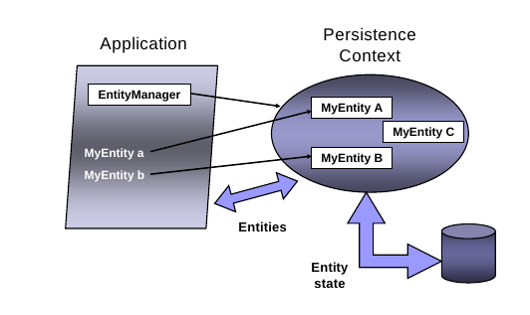
\includegraphics[width=0.95\paperwidth]{img/pic1.png}
\end{frame}


\begin{frame}\frametitle{Entity Manager}
	\begin{itemize}
		\item Client-visible artifact for operating on entities.
        \item API for all the basic persistence operations.
		\item Can think of it as a proxy to a persistence context.
        \item \textbf{May access multiple different persistence contexts throughout its lifetime.}
	\end{itemize}
\begin{tikzpicture}[remember picture,overlay]
    \node[xshift=-0.6cm,yshift=-1.3cm] at (current page.north east){%
    
\includegraphics[width=1cm]{img/pozor}};
\end{tikzpicture}
\end{frame}


\begin{frame}[fragile]\frametitle{Operations on Entities}
Entity manager API
	\begin{itemize}
        \item \verb'persist()' -- insert the state of an entity into the DB (no return value).
        \item \verb'merge()' -- synchronize the state of a detached entity with the PC. \textbf{Returns the managed instance} that the state was merged to.
        \item \verb'remove()' -- delete the entity state from the DB.
        \item \verb'refresh()' -- reload the entity state from the DB.
        \item \verb'find()' -- execute a simple PK query.
        \item \verb'createQuery()' -- create query instance using dynamic JPQL (Java Persistence Query Language).
        \item \verb'createNamedQuery()' -- create an instance for a~predefined query.
        \item \verb'createNativeQuery()' -- create an instance for an SQL query.
        \item \verb'contains()' -- determine if entity is managed by the PC.
        \item \verb'flush()' -- force synchronization of the PC to the database.
	\end{itemize}
\begin{tikzpicture}[remember picture,overlay]
    \node[xshift=-0.6cm,yshift=-1.3cm] at (current page.north east){%
    
\includegraphics[width=1cm]{img/lupa}};
\end{tikzpicture}
\end{frame}


\begin{frame}[fragile]\frametitle{persist()}
	\begin{itemize}
		\item Save the persistent state of the entity and any owned relationship references.
		\item Entity instance becomes managed.
        \medskip
        \item[] \begin{Verbatim}[fontsize=\footnotesize, commandchars=\#\[\]]
public Customer createCust(int id, String name) {
    Customer cust = new Customer(id, name);
    #color[red]#textbf[entityManager.persist(cust);]
    return cust;
}
\end{Verbatim}
	\end{itemize}
\begin{tikzpicture}[remember picture,overlay]
    \node[xshift=-0.6cm,yshift=-1.3cm] at (current page.north east){%
    
\includegraphics[width=1cm]{img/oko}};
\end{tikzpicture}
\end{frame}


\begin{frame}[fragile]\frametitle{find() and remove()}
	\begin{itemize}
		\item \texttt{find()}
          \begin{itemize}
        	\item obtains a managed entity instance with a given persistent identity -- returns \texttt{null} if not found.
          \end{itemize}
        \medskip
        \item \texttt{remove()}
          \begin{itemize}
        	\item deletes a managed entity with the given persistent identity from the database.
          \end{itemize}
        \medskip
        \item[] \begin{Verbatim}[fontsize=\footnotesize, commandchars=\#\[\]]
public void removeCustomer(Long custId) {
    Customer cust =
        #color[red]entityManager.find(Customer.class, custId);
    #color[red]entityManager.remove(cust);
}        
\end{Verbatim}
	\end{itemize}
\end{frame}


\begin{frame}[fragile]\frametitle{Queries}
Overview:
	\renewcommand{\baselinestretch}{1.2}
	\begin{itemize}
		\item Dynamic or statically defined (named queries)
		\item Criteria using JPQL (extension of EJB QL)
		\item Native SQL support (when required)
		\item Named parameters bound at execution time
		\item Pagination and ability to restrict size of result
		\item Single/multiple-entity results, data projections
		\item Bulk update and delete operation on an entity
		\item Standard hooks for vendor-specific hints
	\end{itemize}
    \renewcommand{\baselinestretch}{1.0}
\end{frame}

\begin{frame}[fragile]\frametitle{Queries}
	\begin{itemize}
		\item Query instances are obtained from factory methods on~\texttt{EntityManager}.
		\item Interface \texttt{Query}
        \begin{itemize}
			\item \verb'getResultList()' -- execute query returning multiple results.
            \item \verb'getSingleResult()' -- execute query returning single result.
            \item \verb'executeUpdate()' -- execute bulk update or delete.
            \item \verb'setFirstResult()' -- set the first result to retrieve.
            \item \verb'setMaxResults()' -- set the maximum number of results to~retrieve.
            \item \verb'setParameter()' -- bind a value to a named or positional parameter.
            \item \verb'setHint()' -- apply a vendor-specific hint to the query (\texttt{timeout, cache.retrieveMode, cache.storeMode}, \ldots).
            \item \verb'setFlushMode()' -- apply a flush mode to the query when it gets run.
            \item \ldots
        \end{itemize}
	\end{itemize}
\end{frame}


\begin{frame}\frametitle{Dynamic Queries}
	\begin{itemize}
    	\item Use \texttt{createQuery()} factory method at runtime and pass in the JPQL query string.
    	\item Use correct execution method
          \begin{itemize}
        	\item \texttt{getResultList()}
            \item \texttt{getSingleResult()}
            \item \texttt{executeUpdate()}
            \vspace{.1cm}
          \end{itemize}
    	\item Query may be compiled/checked at creation time or when executed.
    	\item Maximal flexibility for query definition and execution.
	\end{itemize}
\begin{tikzpicture}[remember picture,overlay]
    \node[xshift=-0.6cm,yshift=-1.3cm] at (current page.north east){%
    
\includegraphics[width=1cm]{img/oko}};
\end{tikzpicture}
\end{frame}


\begin{frame}[fragile]\frametitle{Dynamic Queries}
	\begin{itemize}
	\item[]
    	\begin{Verbatim}[fontsize=\footnotesize, commandchars=\#\[\]]
public List findAll(String entityName) {
    return #color[red]entityManager.createQuery(
        #color[red]"select e from " + entityName + " e")
        #color[red].setMaxResults(100)
        #color[red].getResultList();
}
		\end{Verbatim}
      \begin{itemize}
        \item Returns all instances of the given entity type.
	    \item JPQL string contains the entity type. For example, if ``Account'' was passed in, then JPQL string would be: 
        \item[]``\textbf{select e from Account e''}.
      \end{itemize}
	\end{itemize}
\end{frame}


\begin{frame}[fragile]\frametitle{Named Queries}
	\begin{itemize}
		\item[]
        	\begin{Verbatim}[fontsize=\footnotesize, commandchars=\#\[\]]
@NamedQueries({
    #color[red]@NamedQuery(name="Sale.findByCustId",
        #color[red]query="select s from Sale s
            #color[red]where s.customer.id = :custId
            #color[red]order by s.salesDate")})
public class Sale implements Serializable {
...

public List findSalesByCustomer(Customer cust) {
    return
        #color[red]entityManager.createNamedQuery("Sale.findByCustId")
            #color[red].setParameter("custId", cust.getId())
            #color[red].getResultList();
}
			\end{Verbatim}
          \begin{itemize}
            \item  Returns all sales for a given customer.
          \end{itemize}
	\end{itemize}
\begin{tikzpicture}[remember picture,overlay]
    \node[xshift=-0.6cm,yshift=-1.3cm] at (current page.north east){%
    
\includegraphics[width=1cm]{img/oko}};
\end{tikzpicture}
\end{frame}


\begin{frame}\frametitle{Object/Relational Mapping (ORM)}
	\begin{itemize}
		\item ORM maps persistent object state to relational database.
		\item ORM maps relationships to other entities.
		\item Metadata may be annotations or XML (or both).
		\item Annotations
          \begin{itemize}
            \item Physical -- DB tables and columns (e.g. \texttt{@Table}).
        	\item Logical -- object model (e.g. \texttt{@OneToMany}).
          \end{itemize}
		\item XML
          \begin{itemize}
        	\item can additionally specify scoped settings or defaults.
          \end{itemize}
		\item Standard rules for default DB table/column names.
	\end{itemize}
\begin{tikzpicture}[remember picture,overlay]
    \node[xshift=-0.6cm,yshift=-1.3cm] at (current page.north east){%
    
\includegraphics[width=1cm]{img/oko}};
\end{tikzpicture}
\end{frame}


\begin{frame}\frametitle{Simple Mappings}
	\begin{itemize}
		\item Direct mappings of fields/properties to columns
          \begin{itemize}
        	\item \texttt{@Basic} -- optional annotation to indicate simple mapped attribute.
          \end{itemize}
        \item Maps any of the common simple Java types
          \begin{itemize}
        	\item primitives, wrappers, enumerated, serializable, etc.
          \end{itemize}
		\item Used in conjunction with \texttt{@Column}
          \begin{itemize}
            \item allows to have different name for column and corresponding property.
          \end{itemize}
        \item Defaults to the type which is most appropriate if no mapping annotation is present.
		\item It is possible to override any of the defaults.
	\end{itemize}
\end{frame}


\begin{frame}\frametitle{Simple Mappings}
	\centering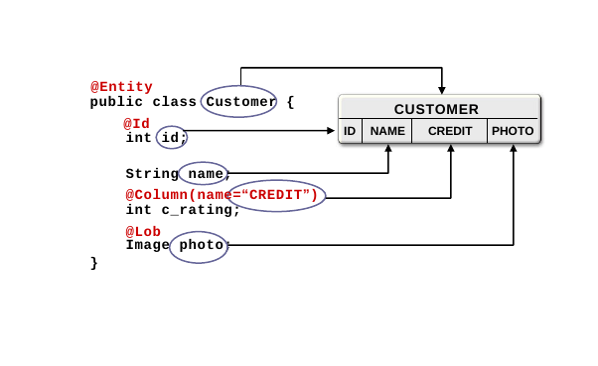
\includegraphics[width=.95\paperwidth]{img/pic2.png}
\begin{tikzpicture}[remember picture,overlay]
    \node[xshift=-0.6cm,yshift=-1.3cm] at (current page.north east){%
    
\includegraphics[width=1cm]{img/lupa}};
\end{tikzpicture}
\end{frame}


\begin{frame}[fragile]\frametitle{Simple Mappings}
\lstset{language=XML}
\begin{lstlisting}
<entity class="com.acme.Customer">
    <attributes>
        <id name="id"/>
        <basic name="c_rating">
            <column name="CREDIT"/>
        </basic>
        <basic name="photo"><lob/></basic>
    </attributes>
</entity>
\end{lstlisting}
\end{frame}


\begin{frame}\frametitle{Relationship Mappings}
	\begin{itemize}
		\item Common relationship mappings supported:
          \begin{itemize}
        	\item \texttt{@ManyToOne}, \texttt{@OneToOne} -- single entity,
        	\item \texttt{@OneToMany}, \texttt{@ManyToMany} -- collection of entities.
          \end{itemize}
		\item Unidirectional or bidirectional.
		\item Every bidirectional relationship have owning and inverse side.
		\item Owning side specifies the physical mapping
        \begin{itemize}
        	\item \texttt{@JoinColumn} to specify foreign key column.
        \end{itemize}
	\end{itemize}
\end{frame}


\begin{frame}\frametitle{ManyToOne Mapping}
	\centering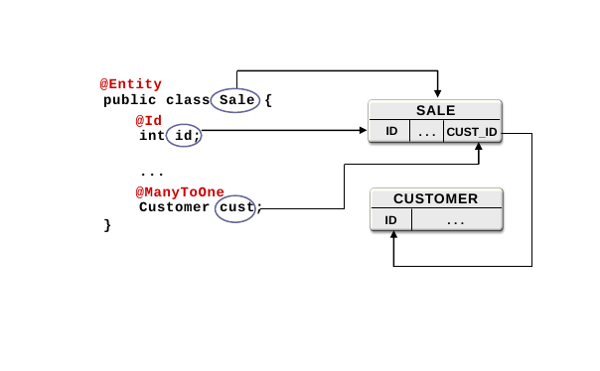
\includegraphics[width=0.95\paperwidth]{img/pic3.png}
\begin{tikzpicture}[remember picture,overlay]
    \node[xshift=-0.6cm,yshift=-1.3cm] at (current page.north east){%
    
\includegraphics[width=1cm]{img/lupa}};
\end{tikzpicture}
\end{frame}


\begin{frame}\frametitle{OneToMany Mapping}
	\centering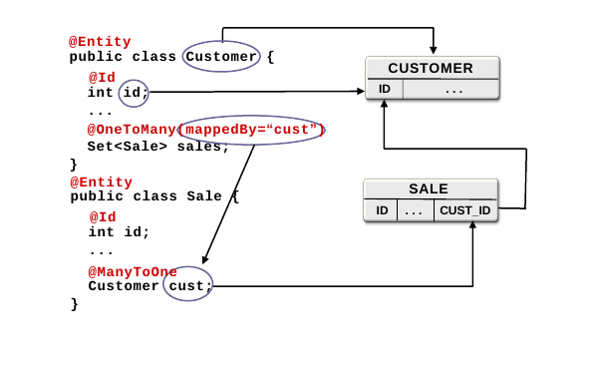
\includegraphics[width=0.95\paperwidth]{img/pic4.png}
\begin{tikzpicture}[remember picture,overlay]
    \node[xshift=-0.6cm,yshift=-1.3cm] at (current page.north east){%
    
\includegraphics[width=1cm]{img/lupa}};
\end{tikzpicture}
\end{frame}


\begin{frame}[fragile]\frametitle{Persistence in Java SE}
	\begin{itemize}
		\item No deployment phase
          \begin{itemize}
            \item We have no \texttt{EntityManagerFactory} from the container.
        	\item Application must use a ``Bootstrap API'' to obtain an \texttt{EntityManagerFactory} (usage of global \texttt{Persistence} object)
            \item[] \verb+ private EntityManagerFactory emFactory = +
            \item[] \verb+   Persistence.createEntityManagerFactory(+
            \item[] \verb+     "persistence-unit-name");+
          \end{itemize}
        \bigskip
		\item Resource-local EntityManager
          \begin{itemize}
        	\item Application uses a local \texttt{EntityTransaction} obtained from the \texttt{EntityManager}.
          \end{itemize}
        \bigskip
		\item New application-managed persistence context for each and every \texttt{EntityManager}.
          \begin{itemize}
        	\item No propagation of persistence contexts.
          \end{itemize}
	\end{itemize}
\begin{tikzpicture}[remember picture,overlay]
    \node[xshift=-0.6cm,yshift=-1.3cm] at (current page.north east){%
    
\includegraphics[width=1cm]{img/oko}};
\end{tikzpicture}
\end{frame}


\begin{frame}\frametitle{Bootstrap Classes}
	\begin{itemize}
		\item \texttt{javax.persistence.Persistence}
          \begin{itemize}
            \item root class for bootstrapping an \texttt{EntityManager},
		    \item locates provider service for a named persistence unit,
		    \item invokes on the provider to obtain an \texttt{EntityManagerFactory}.
          \end{itemize}
		\item \texttt{javax.persistence.EntityManagerFactory}
          \begin{itemize}
            \item Creates \texttt{EntityManager} for a named persistence unit or configuration.
          \end{itemize}
	\end{itemize}
\end{frame}


\begin{frame}\frametitle{Entity Transactions}
	\begin{itemize}
		\item Only used by Resource-local EntityManagers.
		\item Isolated from transactions in other EntityManagers.
		\item Transaction demarcation under explicit application control using interface. \texttt{EntityTransaction}:
        \begin{itemize}
        	\item \texttt{begin()}
            \item \texttt{commit()}
            \item \texttt{rollback()}
            \item \texttt{isActive()}
        \end{itemize}
		\item Underlying (JDBC) resources allocated by \texttt{EntityManager} as required.
	\end{itemize}
\begin{tikzpicture}[remember picture,overlay]
    \node[xshift=-0.6cm,yshift=-1.3cm] at (current page.north east){%
    
\includegraphics[width=1cm]{img/oko}};
\end{tikzpicture}
\end{frame}


\begin{frame}[fragile]\frametitle{Example}
\begin{footnotesize}
persistence.xml
\end{footnotesize}
\lstset{language=XML}
\begin{lstlisting}
<persistence-unit name="jpa-example" transaction-type="RESOURCE_LOCAL">
  <provider>org.hibernate.jpa.HibernatePersistenceProvider</provider>
  <properties>
    <property name="javax.persistence.jdbc.url" 
              value="jdbc:mysql://localhost/jpa_example" />
    <property name="javax.persistence.jdbc.user" 
              value="example" />
    ...
\end{lstlisting}
\lstset{language=Java}
\begin{lstlisting}
public class PersistenceProgram {
    public static void main(String[] args) {
        EntityManagerFactory emf = Persistence
            .createEntityManagerFactory("jpa-example");
        EntityManager em = emf.createEntityManager();
        em.getTransaction().begin();
        // Perform finds, execute queries,
        // update entities, etc.
        em.getTransaction().commit();
        em.close();
        emf.close();
    }
}
\end{lstlisting}
\begin{textblock}{15}(9.0,-0.5)
    {\footnotesize Examples JPA-SE, Guestbook}
\end{textblock}
\end{frame}


\begin{frame}\frametitle{References}
	\begin{itemize}
		\item Java Persistence WikiBook
          \begin{itemize}
        	\item \url{http://en.wikibooks.org/wiki/Java_Persistence}
          \end{itemize}
        \item Documentation
          \begin{itemize}
            \item \url{http://docs.oracle.com/javaee/6/tutorial/doc/bnbpz.html}
          \end{itemize}
        \item Others
          \begin{itemize}
            \item \url{https://dzone.com/articles/jpa-tutorial-setting-jpa-java}
          \end{itemize}
	\end{itemize}
\end{frame}




\bluepage{Hibernate}

\begin{frame}\frametitle{Contents}
  \begin{itemize}
    \item What is Hibernate
	\item Object-relational mapping
	\item Configuration
	\item Annotations
	\item Criteria
	\item Interceptors
  \end{itemize}
\end{frame}

\begin{frame}\frametitle{What is Hibernate}
	\begin{itemize}
		\item Hibernate is an Object-Relational Mapping (ORM) solution for Java.
		\item Open source persistent framework.
		\item Hibernate maps Java classes to the database tables.
		\item Relieves the developer of 95\,\% of common data persistence related programming tasks (according to the documentation).
        \normalsize
        \medskip
        \item[] 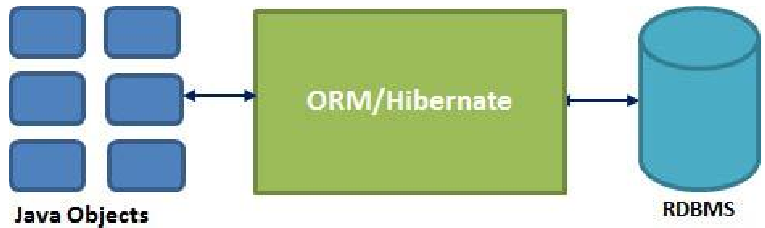
\includegraphics[width=0.8\paperwidth]{img/pic5.png}
	\end{itemize}
\end{frame}


\begin{frame}\frametitle{Hibernate advantages}
	\begin{itemize}
        \item ORM using XML files, without writing a line of code.
        \item Simple API for storing/retrieving Java objects.
        \item Abstract away the unfamiliar SQL types and provide us to work around familiar Java Objects.
		\item Doesn't require running application server.
        \item Minimizes database access with smart fetching strategies.
	\end{itemize}
\end{frame}


\begin{frame}\frametitle{Supported databases}
	\begin{itemize}
		\item HSQL Database Engine
		\item DB2/NT
		\item MySQL
		\item PostgreSQL
		\item FrontBase
		\item Oracle
		\item Microsoft SQL Server Database
		\item Sybase ASE
		\item Informix Dynamic Server
		\item \ldots
	\end{itemize}
\begin{tikzpicture}[remember picture,overlay]
    \node[xshift=-0.6cm,yshift=-1.3cm] at (current page.north east){%
    
\includegraphics[width=1cm]{img/kompas}};
\end{tikzpicture}
\end{frame}


\begin{frame}\frametitle{Hibernate architecture}
	\centering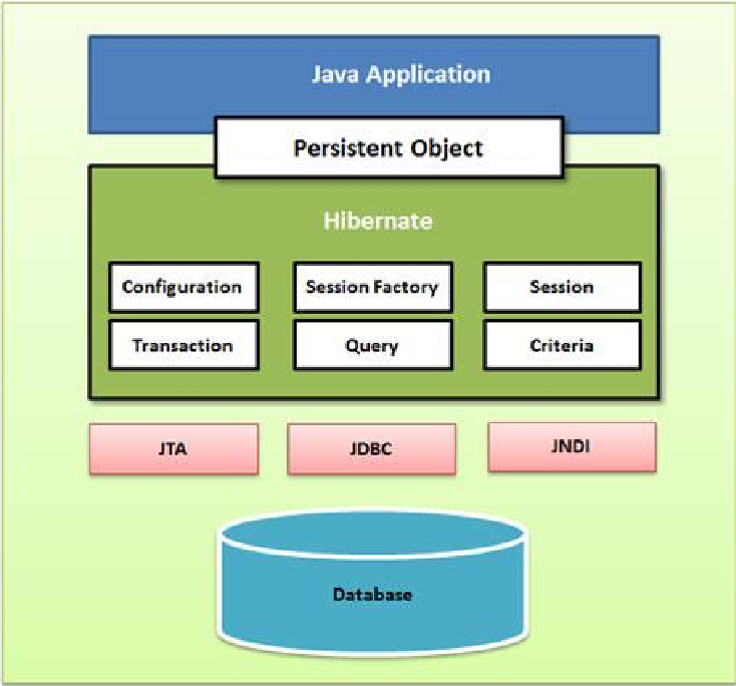
\includegraphics[width=0.7\paperwidth]{img/pic6.png}
\end{frame}

\begin{frame}\frametitle{Hibernate architecture}
 \begin{tikzpicture}[remember picture,overlay]
    \node[xshift=-6.5cm,yshift=-5.5cm] at (current page.north east){%
    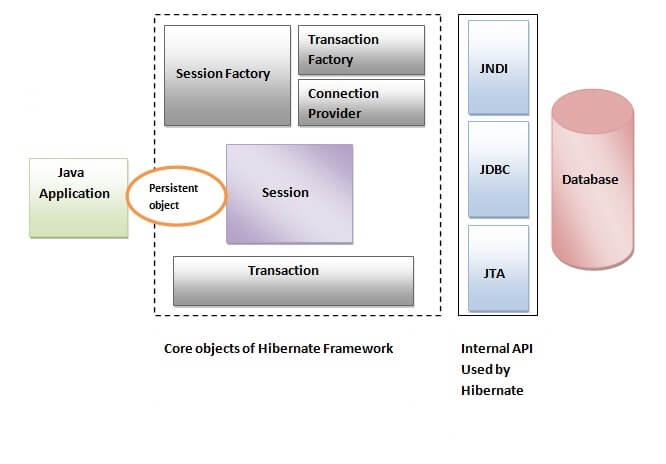
\includegraphics[width=0.95\paperwidth]{img/architecture.jpg}};
\end{tikzpicture}
\end{frame}

\begin{frame}\frametitle{Technologies used by Hibernate}
	\begin{itemize}
		\item Hibernate uses various existing Java APIs, like JDBC, Java Transaction API (JTA) and Java Naming and Directory Interface (JNDI).
        \item JDBC provides a basic level of abstraction of functionality common to the relational databases, allowing almost any database with a JDBC driver to be supported by Hibernate.
        \item JNDI and JTA allows Hibernate to be integrated with JavaEE application servers.
	\end{itemize}
\end{frame}


\begin{frame}\frametitle{Hibernate objects}
	\begin{itemize}
		\item \texttt{Configuration}
          \begin{itemize}
        	\item typically first hibernate object created,
        	\item database connection,
        	\item class mapping setup.
          \end{itemize}
        \item \texttt{SessionFactory}
          \begin{itemize}
        	\item created by configuration object,
        	\item needed one per database.
          \end{itemize}
		\item \texttt{Session}
          \begin{itemize}
        	\item for physical connection with the database.
			\item Persistent objects stored by this object.
          \end{itemize}
		\item \texttt{Transaction}
          \begin{itemize}
        	\item optional, transaction functions from JTA or JDBC.
          \end{itemize}
		\item \texttt{Query}
        \item \texttt{Criteria}
	\end{itemize}
\begin{tikzpicture}[remember picture,overlay]
    \node[xshift=-0.6cm,yshift=-1.3cm] at (current page.north east){%
    
\includegraphics[width=1cm]{img/pozor}};
\end{tikzpicture}
\end{frame}


\begin{frame}\frametitle{Hibernate properties}
	\begin{itemize}
		\item Dialect
          \begin{itemize}
        	\item appropriate SQL for the target database
          \end{itemize}
		\item Connection driver (e.g. JDBC driver for MySQL)
		\item Connection URL
		\item Connection username
		\item Connection password
		\item Pool size
          \begin{itemize}
        	\item number of waiting connections
          \end{itemize}
		\item Autocommit (not recommended) -- specifies when Hibernate should release JDBC connections (default behavior is that connection is held until the session is explicitly closed or disconnected).
	\end{itemize}
\end{frame}


\begin{frame}[fragile]\frametitle{Hibernate.cfg.xml}
\lstset{language=XML}
\begin{lstlisting}
<?xml version="1.0" encoding="utf-8"?>
<!DOCTYPE hibernate-configuration SYSTEM 
    "http://www.hibernate.org/dtd/hibernate-configuration-3.0.dtd">
<hibernate-configuration>
    <session-factory>
        <property name="hibernate.dialect">
            org.hibernate.dialect.MySQLDialect
        </property>
        <property name="hibernate.connection.driver_class">
            com.mysql.cj.jdbc.Driver
	    </property>
        <property name="hibernate.connection.url">
            jdbc:mysql://localhost/test
        </property>
        <property name="hibernate.connection.username">
            test
        </property>
        <property name="hibernate.connection.password">
            test1234
        </property>
        <!-- List of XML mapping files -->
        <mapping resource="Employee.hbm.xml"/>
    </session-factory>
</hibernate-configuration>
\end{lstlisting}
\end{frame}


\begin{frame}[fragile]\frametitle{Mappping configuration file}
	\begin{itemize}
		\item Mappping configuration file is needed for each table.
        \item \texttt{<class>} elements are used to define specific mappings from a Java classes to the database tables.
        \item \texttt{<meta>} element is optional element and can be used to create the class description.
        \item \texttt{<id>} element maps the unique ID attribute in class to the primary key of the database table.
        \item \texttt{<generator>} element within the id element is used to automatically generate the primary key values.
        \item \texttt{<property>} element is used to map a Java class property to the column in the database table.
	\end{itemize}
\end{frame}


\begin{frame}[fragile]\frametitle{Mapping configuration file}
\lstset{language=XML}
\begin{lstlisting}
<?xml version="1.0" encoding="utf-8"?>
<!DOCTYPE hibernate-mapping PUBLIC
    "-//Hibernate/Hibernate Mapping DTD//EN"
    "http://www.hibernate.org/dtd/hibernate-mapping-3.0.dtd">
    <hibernate-mapping>
        <class name="Employee" table="EMPLOYEE">
            <meta attribute="class-description">
                This class contains the employee detail.
            </meta>
            <id name="id" type="int" column="id">
                <generator class="native"/>
            </id>
            <property name="firstName" column="first_name" 
                      type="string"/>
            <property name="lastName" column="last_name" 
                      type="string"/>
            <property name="salary" column="salary" type="int"/>
      </class>
  </hibernate-mapping>
\end{lstlisting}
\end{frame}


\begin{frame}[fragile]\frametitle{Hibernate annotations}
	\begin{itemize}
		\item \texttt{@Entity}
          \begin{itemize}
        	\item must have non-argument constructor,
        	\item denotes entity bean.
          \end{itemize}
		\item \texttt{@Table}
          \begin{itemize}
        	\item allows specifying of details of an entity, that will be persisted in the database.
			\item attributes -- \texttt{name}, \texttt{schema} (namespace), \texttt{catalogue} (named collection of schemas), constraints
            \item[]  \begin{footnotesize}
            \begin{verbatim}
@Entity
@Table(name = "contact", 
    uniqueConstraints = @UniqueConstraint(
        columnNames = {"name", "company_id"}))
public class Contact {
  ...
\end{verbatim}\end{footnotesize}
          \end{itemize}
		\item \texttt{@Id}
          \begin{itemize}
        	\item Each entity bean has a primary key designated by this annotation.
          \end{itemize}
		\item \texttt{@GeneratedValue}
          \begin{itemize}
        	\item Parameter \texttt{strategy}
        	\item Use default generator if possible.
          \end{itemize}
		\item \texttt{@Column}
          \begin{itemize}
        	\item \texttt{name}, \texttt{nullable}, \texttt{unique}
          \end{itemize}
	\end{itemize}
\begin{tikzpicture}[remember picture,overlay]
    \node[xshift=-0.6cm,yshift=-1.3cm] at (current page.north east){%
    
\includegraphics[width=1cm]{img/lupa}};
\end{tikzpicture}
\end{frame}


\begin{frame}[fragile]\frametitle{Hibernate annotations example}
\lstset{language=Java}
\begin{lstlisting}
@Entity
@Table(name = "EMPLOYEE")
public class Employee {

    @Id @GeneratedValue
    @Column(name = "id")
    private int id;

    @Column(name = "first_name")
    private String firstName;

    @Column(name = "last_name")
    private String lastName;

    @Column(name = "salary")
    private int salary;

    ...
}
\end{lstlisting}
\begin{textblock}{15}(8.7,-0.4)
    {\footnotesize Example HibernateAnnotation}
\end{textblock}
\end{frame}


\begin{frame}\frametitle{Hibernate sessions}
	\begin{itemize}
		\itmspace{.4cm} {The main function of the Session is to offer create, read, update and delete operations for instances of mapped entity classes.}
        \item States of instances
          \begin{itemize}
        	\item {\textbf{\emph{transient}} -- A new instance of a persistent class which is not associated with the Session and has no representation in the database and has no identifier value is considered transient by Hibernate.}
        	\item {\textbf{\emph{persistent}} -- You can make a transient instance persistent by associating it with the Session. A persistent instance has a~representation in the database, an identifier value and is~associated with a Session.}
        	\item \textbf{\emph{detached}} -- Once we close the Hibernate Session, the persistent instance will become a detached instance.
          \end{itemize}
	\end{itemize}
\begin{tikzpicture}[remember picture,overlay]
    \node[xshift=-0.6cm,yshift=-1.3cm] at (current page.north east){%
    
\includegraphics[width=1cm]{img/pozor}};
\end{tikzpicture}
\end{frame}


\begin{frame}[fragile]\frametitle{Session methods}
  \begin{itemize}
    \item \texttt{save()}
      \begin{itemize}
        \item persists the given transient instance, first assigning a~generated identifier,
        \item returns the \textbf{generated identifier}.
        \item deprecated -- use \texttt{persist()} instead.
      \end{itemize}
    \item \texttt{persist()}
      \begin{itemize}
        \item persists the given transient instance,
        \item doesn't return an identifier (physical save will be done later),
      \end{itemize}
    \item \texttt{merge()}
      \begin{itemize}
        \item copy the state of the given object onto the persistent object with the same identifier,
        \item returns an updated persistent instance.
      \end{itemize}
    \item \texttt{update()}
      \begin{itemize}
        \item updates the persistent instance with the identifier of the given detached instance.
        \item deprecated -- use \texttt{merge()} instead.
      \end{itemize}
  \end{itemize}
\begin{tikzpicture}[remember picture,overlay]
    \node[xshift=-0.6cm,yshift=-1.3cm] at (current page.north east){%
    
\includegraphics[width=1cm]{img/lupa}};
\end{tikzpicture}
\end{frame}


\begin{frame}[fragile]\frametitle{Session methods}
  \begin{itemize}
    \item \texttt{delete()}
      \begin{itemize}
        \item removes a persistent instance from the datastore,
        \item argument may be an instance associated with the session or a transient instance with an identifier associated with existing persistent state.
        \item Deprecated.
      \end{itemize}
    \item \texttt{remove()}
      \begin{itemize}
        \item removes a persistent instance from the datastore,
        \item argument may be an instance associated with the session or a transient instance with an identifier associated with existing persistent state.
      \end{itemize}
    \item \texttt{contains()}
      \begin{itemize}
        \item checks if this instance is associated with this session.
      \end{itemize}
    \item \texttt{get()}
      \begin{itemize}
        \item returns the persistent instance of the given entity class with the given identifier.
        \item returns the persistent instance of the given named entity with the given identifier.
      \end{itemize}
  \end{itemize}
\end{frame}

\begin{frame}[fragile]\frametitle{Session methods}
  \begin{itemize}
    \item \texttt{flush()}
      \begin{itemize}
        \item forces this session to flush.
      \end{itemize}
    \item \texttt{clear()}
      \begin{itemize}
        \item completely clears the session. Evict all loaded instances and cancels all pending saves, updates and deletions,
        \item frees the memory.
      \end{itemize}
  \end{itemize}
\begin{textblock}{15}(6.1,5.0)
    {\footnotesize Examples HibernateExample, HibernateBatch}
\end{textblock}
\end{frame}


\begin{frame}[fragile]\frametitle{Hibernate query language (HQL)}
	\begin{itemize}
		\item HQL is an object-oriented language, similar to SQL.
		\item Instead of tables and columns HQL works with persisted objects and their properties.
		\item Use HQL whenever possible.
		\item Clauses (similar to SQL)
          \begin{itemize}
        	\item \texttt{FROM} -- loads persistent object to the memory
            \item[]
            	\lstset{language=Java}
                \footnotesize
                \begin{lstlisting}
String hql = "FROM Employee";
Query<Employee> query = session.createQuery(hql, 
                                            Employee.class);
List<Employee> results = query.list();
                \end{lstlisting}
                \normalsize
            \item \texttt{AS} -- optional, aliases in HQL
            \item[]
            	\lstset{language=Java}
                \footnotesize
                \begin{lstlisting}
String hql = "FROM Employee AS E";
Query<Employee> query = session.createQuery(hql, 
                                            Employee.class);
List<Employee> results = query.list();
                \end{lstlisting}
                \normalsize
          \end{itemize}
	\end{itemize}
\begin{tikzpicture}[remember picture,overlay]
    \node[xshift=-0.6cm,yshift=-1.3cm] at (current page.north east){%
    
\includegraphics[width=1cm]{img/oko}};
\end{tikzpicture}
\end{frame}


\begin{frame}[fragile]\frametitle{Hibernate clauses}
	\begin{itemize}
	        \item \texttt{SELECT}
			\item[]
                \begin{footnotesize}
				\lstset{language=Java}
                \begin{lstlisting}
String hql = "SELECT E.firstName FROM Employee E";
Query query = session.createQuery(hql);
List results = query.list();                
                \end{lstlisting} \end{footnotesize}
			\item \texttt{WHERE}
			\item[]
                \begin{footnotesize}
				\lstset{language=Java}
                \begin{lstlisting}
String hql = "FROM Employee E WHERE E.id = 10";
Query query = session.createQuery(hql);
List results = query.list();                
                \end{lstlisting} \end{footnotesize}
            \item \texttt{ORDER BY}
			\item[]
				\begin{footnotesize}
                \lstset{language=Java}
                \begin{lstlisting}
String hql = "FROM Employee E WHERE E.id > 10 " + 
             "ORDER BY E.salary DESC";
Query query = session.createQuery(hql);
List results = query.list();                
                \end{lstlisting} \end{footnotesize}
            \item \texttt{GROUP BY}
            \item[]
				\begin{footnotesize}
                \lstset{language=Java}
                \begin{lstlisting}
String hql = "SELECT SUM(E.salary), E.firstName " +
             "FROM Employee E " +
             "GROUP BY E.firstName";
Query query = session.createQuery(hql);
List results = query.list();                
                \end{lstlisting} \end{footnotesize}
                \normalsize            
	\end{itemize}
\end{frame}


\begin{frame}[fragile]\frametitle{Hibernate clauses}
	\begin{itemize}
		\item Using named paramaters
          \begin{itemize}
            \item no need to defend SQL injection
          \end{itemize}
        \item[] \footnotesize \lstset{language=Java}
                \begin{lstlisting}   
String hql = "FROM Employee E WHERE E.id = :employee_id";
Query query = session.createQuery(hql);
query.setParameter("employee_id",10);
List results = query.list();                
                \end{lstlisting}            
    \end{itemize}
\end{frame}


\begin{frame}[fragile]\frametitle{Hibernate clauses}
	\begin{itemize}
    	\item \texttt{INSERT}
        \item[]
            \begin{footnotesize}
            \lstset{language=Java}
            \begin{lstlisting}         
String hql = 
    "INSERT INTO Employee(firstName, lastName, salary) " + 
    "SELECT firstName, lastName, salary FROM old_employee";
Query query = session.createQuery(hql);
int result = query.executeUpdate(); // returns the number 
                                    // of entities updated 
                                    // or deleted
            \end{lstlisting} \end{footnotesize}
		\item \texttt{UPDATE}
        \item[]
        	\begin{footnotesize}
			\lstset{language=Java}
            \begin{lstlisting}        
String hql = "UPDATE Employee set salary = :salary " + 
             "WHERE id = :employee_id";
Query query = session.createQuery(hql);
query.setParameter("salary", 1000);
query.setParameter("employee_id", 10);
int result = query.executeUpdate();
            \end{lstlisting} \end{footnotesize}
		\item \texttt{DELETE}
        \item[]
            \begin{footnotesize}
			\lstset{language=Java}
            \begin{lstlisting}   
String hql = "DELETE FROM Employee " + 
             "WHERE id = :employee_id";
Query query = session.createQuery(hql);
query.setParameter("employee_id", 10);
int result = query.executeUpdate();
            \end{lstlisting} \end{footnotesize}
	\end{itemize}
\end{frame}


\begin{frame}[fragile]\frametitle{Aggregate methods and pagination}
	\begin{itemize}
		\item Aggregate functions
          \begin{itemize}
        	\item \texttt{avg}
            \item \texttt{count}
            \item \texttt{max}
            \item \texttt{min}
            \item \texttt{sum}
            \item[]
                \begin{footnotesize}
                \lstset{language=Java}
                \begin{lstlisting}    
String hql = "SELECT count(distinct E.firstName) FROM Employee E";
Query query = session.createQuery(hql);
List results = query.list();                
                \end{lstlisting}  
                \end{footnotesize}
          \end{itemize}
		\item Pagination
          \begin{itemize}
        	\item \inlinejava{setFirstResult(int startPosition)}
        	\item \inlinejava{setMaxResults(int maxResults)}
            \item[]
                \begin{footnotesize}
                \lstset{language=Java}
                \begin{lstlisting}     
String hql = "FROM Employee";
Query query = session.createQuery(hql);
query.setFirstResult(1);
query.setMaxResults(10);
List results = query.list();                
                \end{lstlisting}  
                \end{footnotesize}
          \end{itemize}
	\end{itemize}
\end{frame}


\begin{frame}[fragile]\frametitle{Hibernate criteria}
	\begin{itemize}
		\item Criteria are very useful method for restricting of results
		\item[]
        	\footnotesize
            \lstset{language=Java}
            \begin{lstlisting}            
Criteria cr = session.createCriteria(Employee.class);
List results = cr.list();            
			\end{lstlisting}  
            \normalsize
        \medskip
		\item Put some constraints on result set
		\item[]
        	\footnotesize
            \lstset{language=Java}
            \begin{lstlisting}  
// To get records having salary more than 2000
cr.add(Restrictions.gt("salary", 2000));
// To get records having salary less than 2000
cr.add(Restrictions.lt("salary", 2000));
// To get records having fistName starting with mary
cr.add(Restrictions.like("firstName", "mary%"));
// Case insensitive form of the above restriction.
cr.add(Restrictions.ilike("firstName", "mary%"));
// To get records having salary in between 1000 and 2000
cr.add(Restrictions.between("salary", 1000, 2000));
// To check if the given property is null
cr.add(Restrictions.isNull("salary"));
// To check if the given property is not null
cr.add(Restrictions.isNotNull("salary"));
// To check if the given property is empty
cr.add(Restrictions.isEmpty("salary"));
// To check if the given property is not empty
cr.add(Restrictions.isNotEmpty("salary"));            
			\end{lstlisting}  
            \normalsize
	\end{itemize}
\begin{tikzpicture}[remember picture,overlay]
    \node[xshift=-0.6cm,yshift=-1.3cm] at (current page.north east){%
    
\includegraphics[width=1cm]{img/oko}};
\end{tikzpicture}
\end{frame}


\begin{frame}[fragile]\frametitle{Hibernate criteria}
	\begin{itemize}
		\item Sorting
        \item[]
			\footnotesize
          	\begin{tabular}{l p{6cm}}	
				$\circ\ $ \emph{Ascending} &
                \verb'cr.addOrder(Order.asc("salary"))'\\[.1cm]
				$\circ\ $ \emph{Descending} & 				
                \verb'cr.addOrder(Order.desc("salary"))'
          	\end{tabular}
          	\normalsize
        \medskip
		\item Projections $\mathcal{\&}$ aggregations
		\item[]
        	\footnotesize
            \lstset{language=Java}
            \begin{lstlisting}    
Criteria cr = session.createCriteria(Employee.class);
// To get total row count.
cr.setProjection(Projections.rowCount());

// To get average of a property.
cr.setProjection(Projections.avg("salary"));

// To get distinct count of a property.
cr.setProjection(Projections.countDistinct("firstName"));

// To get maximum of a property.
cr.setProjection(Projections.max("salary"));

// To get minimum of a property.
cr.setProjection(Projections.min("salary"));

// To get sum of a property.
cr.setProjection(Projections.sum("salary"));
			\end{lstlisting}  
            \normalsize        
	\end{itemize}
\begin{textblock}{15}(9.3,-0.2)
    {\footnotesize Example HibernateCriteria}
\end{textblock}
\begin{tikzpicture}[remember picture,overlay]
    \node[xshift=-0.6cm,yshift=-1.3cm] at (current page.north east){%
    
\includegraphics[width=1cm]{img/oko}};
\end{tikzpicture}
\end{frame}


\begin{frame}[fragile]\frametitle{Hibernate criteria}
	\begin{itemize}
		\item Criteria are deprecated, and removed in the newest version.
        \item We can replace Criteria by
        \item[] \texttt{jakarta.persistence.criteria.CriteriaBuilder}
        \item[] \texttt{jakarta.persistence.criteria.CriteriaQuery}
        \item[] \footnotesize
                \lstset{language=Java}
                \begin{lstlisting}   
CriteriaBuilder cb = session.getCriteriaBuilder();
// To get total row count
CriteriaQuery<Long> cq = cb.createQuery(Long.class);
Root<Employee> root = cq.from(Employee.class);
cq.select(cb.count(root));
Long count = session.createQuery(cq).getSingleResult();        
                \end{lstlisting}  
                \normalsize  
        \item Some functionality was removed
        \item[] {\footnotesize \verb+query.setResultTransformer(Criteria.ALIAS_TO_ENTITY_MAP);+}
	\end{itemize}
\begin{textblock}{15}(9.3,1.6)
    {\footnotesize Example HibernateBatch}
\end{textblock}
\end{frame}


\begin{frame}[fragile]\frametitle{Hibernate Native SQL}
	\begin{itemize}
		\item Scalar query
          \begin{itemize}
        	\item the most basic SQL query
            \item[]
                \footnotesize
                \lstset{language=Java}
                \begin{lstlisting}   
String sql = "SELECT first_name, salary FROM EMPLOYEE";
SQLQuery query = session.createSQLQuery(sql);
query.setResultTransformer(Criteria.ALIAS_TO_ENTITY_MAP);
List results = query.list();                
                \end{lstlisting}  
                \normalsize             
          \end{itemize}
		\item Entity query
          \begin{itemize}
        	\item selects raw values from the resultset
            \item[]
                \footnotesize
                \lstset{language=Java}
                \begin{lstlisting}   
String sql = "SELECT * FROM EMPLOYEE";
SQLQuery query = session.createSQLQuery(sql);
query.addEntity(Employee.class);
List results = query.list();                
                \end{lstlisting}  
                \normalsize             
          \end{itemize}
		\item Parameters
        \item[]
        	\footnotesize
            \lstset{language=Java}
            \begin{lstlisting}  
String sql = "SELECT * FROM EMPLOYEE WHERE " +
             "id = :employee_id";
SQLQuery query = session.createSQLQuery(sql);
query.addEntity(Employee.class);
query.setParameter("employee_id", 10);
List results = query.list();            
			\end{lstlisting}  
            \normalsize  
	\end{itemize}
\begin{textblock}{15}(9.5,-0.3)
    {\footnotesize Example HibernateNative}
\end{textblock}
\end{frame}


\begin{frame}[fragile]\frametitle{Hibernate Native SQL}
	\begin{itemize}
        \item Named SQL queries
        \item[]
        	\footnotesize
            \lstset{language=Java}
            \begin{lstlisting}   
List employees = sess.getNamedQuery("employees")
    .setString("namePattern", namePattern)
    .list();            
			\end{lstlisting}  
            \normalsize        
	\end{itemize}
\end{frame}

\begin{frame}[fragile]\frametitle{Hibernate Native SQL}
  \begin{itemize}
    \item \texttt{SQLQuery} is deprecated.
    \item We can replace it by \texttt{NativeQuery}.
  \end{itemize}
\begin{textblock}{15}(5.9,6.6)
    {\footnotesize Examples HibernateNative2, HibernateNative3}
\end{textblock}
\end{frame}


\begin{frame}\frametitle{Hibernate caching}
        \begin{itemize}
        	\item First level cache
              \begin{itemize}
            	\item everything goes 
                \item[] through it
				\item mandatory
              \end{itemize}
            \medskip
			\item Second level cache
              \begin{itemize}
            	\item per class 
                \item[] or per collection
            	\item optional
              \end{itemize}
            \medskip
			\item Query cache
              \begin{itemize}
            	\item for often  
                \item[] performed queries
              \end{itemize}
        \end{itemize}

        \putat{120}{-5}{
    	    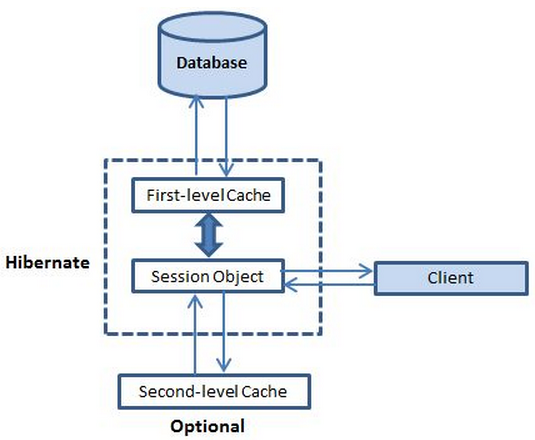
\includegraphics[trim={0 0 .15cm 0}, clip, width=0.58\paperwidth]{img/pic7.png}
        }
\begin{tikzpicture}[remember picture,overlay]
    \node[xshift=-0.6cm,yshift=-1.3cm] at (current page.north east){%
    
\includegraphics[width=1cm]{img/pozor}};
\end{tikzpicture}
\end{frame}


\begin{frame}[fragile]\frametitle{Hibernate interceptors}
	\begin{itemize}
		\item Object goes through different stages per lifecycle.
		\item Interceptors are callbacks when going through these stages.
		\item Creating interceptor
          \begin{itemize}
        	\item either implement \texttt{Interceptor} manually
        	\item or extend class \inlinejava{EmptyInterceptor} (deprecated)
          \end{itemize}
        \smallskip
		\item Methods
          \begin{itemize}
        	\item \inlinejava{findDirty()} -- {\footnotesize called from \texttt{flush()}, returns whether the entity is~updated (an array of dirty property indices)}.
        	\item \verb+instantiate(String entityName,+
            \item[] \verb+         EntityMode entityMode, // POJO/DOM4J/MAP+
            \item[] \verb+         Serializable id)+
        	\item \inlinejava{onDelete()} -- {\footnotesize called before an object is deleted.}
        	\item \inlinejava{onFlushDirty()} -- {\footnotesize object is detected to be dirty, during a flush.}
        	\item \inlinejava{onLoad()} -- {\footnotesize an object is initialized.}
        	\item \inlinejava{onSave()} -- {\footnotesize before an object is saved.}
        	\item \inlinejava{postFlush()}
        	\item \inlinejava{preFlush()}
            \item \ldots
          \end{itemize}
		\normalsize
	\end{itemize}
\begin{textblock}{15}(8.7,-0.3)
    {\footnotesize Example HibernateInterceptor}
\end{textblock}
\end{frame}

\begin{frame}\frametitle{References}
	\begin{itemize}
		\item \url{http://www.tutorialspoint.com/hibernate}
		\item \url{https://docs.jboss.org/hibernate/orm/3.6/javadocs/}
        \item \url{https://docs.jboss.org/hibernate/orm/5.4/javadocs/}
        \item \url{https://docs.jboss.org/hibernate/orm/6.0/}
        \item \url{https://docs.jboss.org/hibernate/orm/6.3/javadocs/}
        \item \url{http://docs.jboss.org/hibernate/orm/3.6/reference/en-US/html/}
        \item \url{https://docs.jboss.org/hibernate/orm/5.4/userguide/html_single/Hibernate_User_Guide.html}
        \item \url{https://docs.jboss.org/hibernate/orm/5.4/quickstart/html_single/}
        \item \url{http://blog.eyallupu.com/2011/01/hibernatejpa-identity-generators.html}
	\end{itemize}
\end{frame}

\begin{frame}\frametitle{References}
	\begin{itemize}
        \item \url{https://developer.jboss.org/docs/DOC-13953}
        \item \url{https://www.baeldung.com/hibernate-criteria-queries}
        \item \url{https://vladmihalcea.com/why-should-not-use-the-auto-jpa-generationtype-with-mysql-and-hibernate/}
        \item \url{https://www.javatpoint.com/hibernate-architecture}
	\end{itemize}
\end{frame}


\bluepage{Thank you for your attention!}



\end{document}
